%=====================================================
\begin{frame}{2.1.1. Признание ценности сотрудничества и доверия (сводный результат) }


\tiny

На диаграмме представлен сводный результат по вопросам Б13, Б14:
\bigskip

Б13. Наличие профессиональных задач, для решения которых требуется знакомство с опытом работы коллег: ``Есть ли у Вас профессиональные задачи, решение которых требует знакомства с опытом работы других педагогов (преподавателей, воспитателей) Вашей образовательной организации?''
\smallskip

Б14. Полезность и правильность посещения педагогами  занятий и мероприятий, проводимых другими: ``Считаете ли Вы полезным и правильным посещение педагогами (преподавателями, воспитателями)  занятий и мероприятий (не открытых, т.е. специально не подготовленных), проводимых другими?''
\bigskip

\begin{columns}
\begin{column}{0.4\textwidth} 
\centering
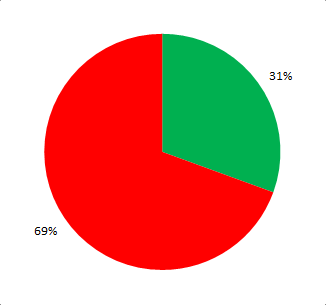
\includegraphics[width=4cm, height=4cm]{diag.png}
\end{column}
\begin{column}{0.6\textwidth} \begin{tabular}{l} 
 Ответили утвердительно   \\ 
(``да'' или ``скорее да, чем нет'')  ---   \numExpC\ (33\%) \\ [0.3cm]
 Ответили отрицательно  \\ 
 (``нет'' или ``скорее нет, чем да'') ---  \numExpD\ (67\%) \\ 
\end{tabular}
\end{column}
\end{columns}

\end{frame}


